% The five Platonic solids (orthographic wireframes, hidden edges dashed) with the orders of their rotation groups. Generated by a short script.
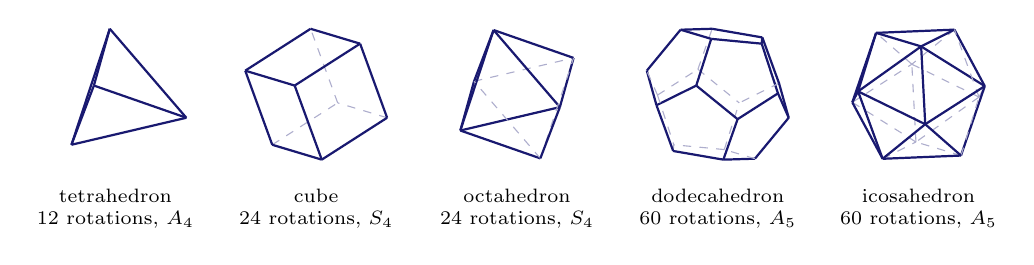
\begin{tikzpicture}[font=\scriptsize]
\draw[MidnightBlue,thick] (0.901,-0.299) -- (-0.071,0.831);
\draw[MidnightBlue,thick] (-0.558,-0.642) -- (-0.071,0.831);
\draw[MidnightBlue,thick] (-0.558,-0.642) -- (0.901,-0.299);
\draw[MidnightBlue,thick] (-0.273,0.110) -- (-0.071,0.831);
\draw[MidnightBlue,thick] (-0.273,0.110) -- (0.901,-0.299);
\draw[MidnightBlue,thick] (-0.273,0.110) -- (-0.558,-0.642);
\node[align=center] at (0.00,-1.45) {tetrahedron\\$12$ rotations, $A_4$};
\draw[MidnightBlue!35,dashed] (2.823,-0.110) -- (2.479,0.831);
\draw[MidnightBlue,thick] (3.108,0.642) -- (2.479,0.831);
\draw[MidnightBlue!35,dashed] (3.451,-0.299) -- (2.823,-0.110);
\draw[MidnightBlue,thick] (3.451,-0.299) -- (3.108,0.642);
\draw[MidnightBlue,thick] (1.649,0.299) -- (2.479,0.831);
\draw[MidnightBlue!35,dashed] (1.992,-0.642) -- (2.823,-0.110);
\draw[MidnightBlue,thick] (1.992,-0.642) -- (1.649,0.299);
\draw[MidnightBlue,thick] (2.277,0.110) -- (3.108,0.642);
\draw[MidnightBlue,thick] (2.277,0.110) -- (1.649,0.299);
\draw[MidnightBlue,thick] (2.621,-0.831) -- (3.451,-0.299);
\draw[MidnightBlue,thick] (2.621,-0.831) -- (1.992,-0.642);
\draw[MidnightBlue,thick] (2.621,-0.831) -- (2.277,0.110);
\node[align=center] at (2.55,-1.45) {cube\\$24$ rotations, $\mathfrak S_4$};
\draw[MidnightBlue!35,dashed] (4.555,0.164) -- (5.819,0.461);
\draw[MidnightBlue,thick] (4.555,0.164) -- (4.381,-0.461);
\draw[MidnightBlue,thick] (5.645,-0.164) -- (5.819,0.461);
\draw[MidnightBlue,thick] (5.645,-0.164) -- (4.381,-0.461);
\draw[MidnightBlue,thick] (4.803,0.815) -- (5.819,0.461);
\draw[MidnightBlue,thick] (4.803,0.815) -- (4.381,-0.461);
\draw[MidnightBlue,thick] (4.803,0.815) -- (4.555,0.164);
\draw[MidnightBlue,thick] (4.803,0.815) -- (5.645,-0.164);
\draw[MidnightBlue!35,dashed] (5.397,-0.815) -- (5.819,0.461);
\draw[MidnightBlue,thick] (5.397,-0.815) -- (4.381,-0.461);
\draw[MidnightBlue!35,dashed] (5.397,-0.815) -- (4.555,0.164);
\draw[MidnightBlue,thick] (5.397,-0.815) -- (5.645,-0.164);
\node[align=center] at (5.10,-1.45) {octahedron\\$24$ rotations, $\mathfrak S_4$};
\draw[MidnightBlue,thick] (7.178,0.819) -- (7.579,0.831);
\draw[MidnightBlue,thick] (7.178,0.819) -- (6.749,0.299);
\draw[MidnightBlue!35,dashed] (7.398,0.317) -- (7.579,0.831);
\draw[MidnightBlue!35,dashed] (7.398,0.317) -- (7.923,-0.110);
\draw[MidnightBlue,thick] (8.216,0.721) -- (7.579,0.831);
\draw[MidnightBlue,thick] (8.216,0.721) -- (8.208,0.642);
\draw[MidnightBlue!35,dashed] (7.733,-0.703) -- (7.923,-0.110);
\draw[MidnightBlue!35,dashed] (7.733,-0.703) -- (7.092,-0.642);
\draw[MidnightBlue,thick] (8.415,0.011) -- (8.208,0.642);
\draw[MidnightBlue,thick] (8.415,0.011) -- (8.551,-0.299);
\draw[MidnightBlue,thick] (6.872,-0.140) -- (6.749,0.299);
\draw[MidnightBlue,thick] (6.872,-0.140) -- (7.377,0.110);
\draw[MidnightBlue,thick] (7.567,0.703) -- (8.208,0.642);
\draw[MidnightBlue,thick] (7.567,0.703) -- (7.377,0.110);
\draw[MidnightBlue,thick] (7.567,0.703) -- (7.178,0.819);
\draw[MidnightBlue!35,dashed] (6.885,-0.011) -- (6.749,0.299);
\draw[MidnightBlue!35,dashed] (6.885,-0.011) -- (7.092,-0.642);
\draw[MidnightBlue!35,dashed] (6.885,-0.011) -- (7.398,0.317);
\draw[MidnightBlue!35,dashed] (8.428,0.140) -- (7.923,-0.110);
\draw[MidnightBlue,thick] (8.428,0.140) -- (8.551,-0.299);
\draw[MidnightBlue,thick] (8.428,0.140) -- (8.216,0.721);
\draw[MidnightBlue,thick] (8.122,-0.819) -- (8.551,-0.299);
\draw[MidnightBlue,thick] (8.122,-0.819) -- (7.721,-0.831);
\draw[MidnightBlue!35,dashed] (8.122,-0.819) -- (7.733,-0.703);
\draw[MidnightBlue,thick] (7.902,-0.317) -- (7.377,0.110);
\draw[MidnightBlue,thick] (7.902,-0.317) -- (7.721,-0.831);
\draw[MidnightBlue,thick] (7.902,-0.317) -- (8.415,0.011);
\draw[MidnightBlue!35,dashed] (7.084,-0.721) -- (7.092,-0.642);
\draw[MidnightBlue,thick] (7.084,-0.721) -- (7.721,-0.831);
\draw[MidnightBlue,thick] (7.084,-0.721) -- (6.872,-0.140);
\node[align=center] at (7.65,-1.45) {dodecahedron\\$60$ rotations, $A_5$};
\draw[MidnightBlue!35,dashed] (10.115,0.381) -- (9.661,0.779);
\draw[MidnightBlue,thick] (10.656,0.820) -- (9.661,0.779);
\draw[MidnightBlue!35,dashed] (10.656,0.820) -- (10.115,0.381);
\draw[MidnightBlue!35,dashed] (10.167,-0.607) -- (10.115,0.381);
\draw[MidnightBlue,thick] (11.041,0.103) -- (10.656,0.820);
\draw[MidnightBlue,thick] (9.432,0.036) -- (9.661,0.779);
\draw[MidnightBlue,thick] (10.233,0.607) -- (9.661,0.779);
\draw[MidnightBlue,thick] (10.233,0.607) -- (10.656,0.820);
\draw[MidnightBlue,thick] (10.233,0.607) -- (11.041,0.103);
\draw[MidnightBlue,thick] (10.233,0.607) -- (9.432,0.036);
\draw[MidnightBlue,thick] (9.359,-0.103) -- (9.661,0.779);
\draw[MidnightBlue!35,dashed] (9.359,-0.103) -- (10.115,0.381);
\draw[MidnightBlue!35,dashed] (9.359,-0.103) -- (10.167,-0.607);
\draw[MidnightBlue,thick] (9.359,-0.103) -- (9.432,0.036);
\draw[MidnightBlue!35,dashed] (10.968,-0.036) -- (10.115,0.381);
\draw[MidnightBlue!35,dashed] (10.968,-0.036) -- (10.656,0.820);
\draw[MidnightBlue!35,dashed] (10.968,-0.036) -- (10.167,-0.607);
\draw[MidnightBlue!35,dashed] (10.968,-0.036) -- (11.041,0.103);
\draw[MidnightBlue!35,dashed] (10.739,-0.779) -- (10.167,-0.607);
\draw[MidnightBlue,thick] (10.739,-0.779) -- (11.041,0.103);
\draw[MidnightBlue!35,dashed] (10.739,-0.779) -- (10.968,-0.036);
\draw[MidnightBlue,thick] (10.285,-0.381) -- (11.041,0.103);
\draw[MidnightBlue,thick] (10.285,-0.381) -- (9.432,0.036);
\draw[MidnightBlue,thick] (10.285,-0.381) -- (10.233,0.607);
\draw[MidnightBlue,thick] (10.285,-0.381) -- (10.739,-0.779);
\draw[MidnightBlue!35,dashed] (9.744,-0.820) -- (10.167,-0.607);
\draw[MidnightBlue,thick] (9.744,-0.820) -- (9.432,0.036);
\draw[MidnightBlue,thick] (9.744,-0.820) -- (9.359,-0.103);
\draw[MidnightBlue,thick] (9.744,-0.820) -- (10.739,-0.779);
\draw[MidnightBlue,thick] (9.744,-0.820) -- (10.285,-0.381);
\node[align=center] at (10.20,-1.45) {icosahedron\\$60$ rotations, $A_5$};
\end{tikzpicture}
